\section{The Transformer Architecture}
\label{sec:transformer}

The architecture Vaswani et al. proposed is composed of two parts \cite{vaswaniAttentionAllYou2023}, \cite[Chap.~25]{russellArtificialIntelligenceModern2022}:
\begin{itemize}
    \item the \emph{encoder} maps the input sequence to a sequence of internal representations;
    \item the \emph{decoder} produces an output sequence, predicting each token from the encoder output and from the tokens already generated.
\end{itemize}

Current generative language models are decoder-only, comprising the decoder part alone, which predicts the next token from the preceding ones without a separate encoder \cite[Chap.~25]{russellArtificialIntelligenceModern2022}. With no encoder to hold a separate input sequence, the query and the tokens generated so far occupy positions of the same single sequence. Generation is autoregressive: each emitted token is appended to that sequence before the next one is predicted \cite{zhaoSurveyLargeLanguage2026}. The number of preceding tokens a prediction can use is fixed and is defined as the context window \cite{zhaoSurveyLargeLanguage2026}. The models used in this work are of this kind, and the remainder of this section describes one call to a decoder-only model, one step at a time: the query is segmented into tokens, the tokens are converted into vectors, a stack of identical blocks transforms these vectors into a new vector per token position, and the vector at the last position is converted into the distribution from which the emitted token is selected.

\subsection{Tokens}
\label{subsec:tokens}

\emph{Tokens} are the units of a fixed vocabulary into which text is segmented before it is processed \cite{zhaoSurveyLargeLanguage2026}. Tokenization is performed by subword methods, which keep frequent words as single units and split rarer ones into smaller pieces, so that any input can be represented with a vocabulary of bounded size \cite{zhaoSurveyLargeLanguage2026}, \cite[Chap.~24]{russellArtificialIntelligenceModern2022}. A token is therefore not a linguistic unit, and one word can correspond to several tokens. Everything the model reads and everything it emits is a sequence of tokens, and the positions referred to throughout this chapter are token positions.

As an example, Table~\ref{tab:tokenization-example} shows how a byte-pair-encoding tokenizer segments the word \texttt{unbelievability} into four tokens. The boundaries do not follow the parts of the word that carry meaning: \emph{unbelievability} is split with \texttt{v} separated from \texttt{belie} rather than kept together as \texttt{believ}.

\begin{table}[ht]
    \centering
    \renewcommand{\arraystretch}{1.2}
    \begin{tabular}{@{}ll@{}}
        \toprule
        Token ID & Token text \\
        \midrule
        359 & \texttt{un} \\
        32898 & \texttt{belie} \\
        85 & \texttt{v} \\
        2968 & \texttt{ability} \\
        \bottomrule
    \end{tabular}
    \caption[Tokenization of \texttt{unbelievability} by a byte-pair-encoding tokenizer]{Tokenization of \texttt{unbelievability} by a byte-pair-encoding tokenizer.}
    \label{tab:tokenization-example}
\end{table}

\subsection{Embedding: tokens to vectors}
\label{subsec:embedding}

Each token of the vocabulary is associated with a learned vector of dimension $d_{\mathrm{model}}$. The input sequence is converted into the corresponding sequence of vectors before it reaches the first block \cite{vaswaniAttentionAllYou2023}. Attention, defined in Section~\ref{subsec:attention}, relates any two positions with the same operation regardless of where they occur in the sequence, so it carries no notion of order on its own. Information about the position of each token is therefore supplied separately and combined with the token vector, so that two identical tokens at different positions do not enter the stack with the same representation \cite{vaswaniAttentionAllYou2023}. This added information is called the \emph{positional encoding} \cite{vaswaniAttentionAllYou2023}. The result is one vector per token position, which is the input of the first block.

Table~\ref{tab:positional-encoding-example} shows this combination for the four tokens of \texttt{unbelievability} from Table~\ref{tab:tokenization-example}.

\begin{table}[H]
  \centering
  \renewcommand{\arraystretch}{1.2}
  \begin{tabular}{@{}lccc@{}}
    \toprule
    Token & Token embedding & Positional encoding & Input vector \\
    \midrule
    \texttt{un}      & $e_{\mathtt{un}}$      & $p_1$ & $e_{\mathtt{un}} + p_1$ \\
    \texttt{belie}   & $e_{\mathtt{belie}}$   & $p_2$ & $e_{\mathtt{belie}} + p_2$ \\
    \texttt{v}       & $e_{\mathtt{v}}$       & $p_3$ & $e_{\mathtt{v}} + p_3$ \\
    \texttt{ability} & $e_{\mathtt{ability}}$ & $p_4$ & $e_{\mathtt{ability}} + p_4$ \\
    \bottomrule
  \end{tabular}
  \caption[Positional encoding example for \texttt{unbelievability}]{Positional encoding example for \texttt{unbelievability}.}
  \label{tab:positional-encoding-example}
\end{table}

\subsection{Attention}
\label{subsec:attention}

Attention is a mechanism that computes, for each pair of tokens, a weight reflecting their relevance to each other \cite{vaswaniAttentionAllYou2023}, \cite[Chap.~25]{russellArtificialIntelligenceModern2022}. Each token is then represented as a sum of the representations of every other token, weighted by these values. This sum includes a distant token's representation in the same step as a neighboring one's, unlike the recurrent computation of Section~\ref{subsec:counting-to-learned}, where information about a distant token has to pass through the representation of every token between it and the current position \cite{vaswaniAttentionAllYou2023}.

The mechanism operates on three sets of vectors derived from the token representations, the queries, keys, and values \cite{vaswaniAttentionAllYou2023}. With these arranged into matrices $Q$, $K$, and $V$, scaled dot-product Attention is computed as
\begin{equation}
    \mathrm{Attention}(Q, K, V) = \mathrm{softmax}\!\left(\frac{QK^\top}{\sqrt{d_k}}\right) V ,
\end{equation}
where $d_k$ is the dimension of the queries and keys \cite{vaswaniAttentionAllYou2023}. Each operation in the expression has a distinct role:
\begin{itemize}
    \item the product $QK^\top$ scores each query against every key through their dot product;
    \item the division by $\sqrt{d_k}$ prevents the scores from growing too large, which would push the softmax into a region where its gradients are too small for training to proceed \cite{vaswaniAttentionAllYou2023};
    \item the softmax normalizes the scores into weights that sum to one, so that each output is the corresponding weighted sum of the values \cite{vaswaniAttentionAllYou2023}.
\end{itemize}
In the Transformer architecture, this computation is carried out in parallel by several Attention heads, each operating over a distinct learned subspace, so that different relations between tokens can be represented simultaneously \cite{vaswaniAttentionAllYou2023}. $Q$, $K$, and $V$ are each projected by a separate learned matrix per head, $h$ instances of scaled dot-product Attention are computed independently, one per head, and the resulting vectors are concatenated and projected once more:
\begin{equation}
    \mathrm{MultiHead}(Q, K, V) = \mathrm{Concat}(\mathrm{head}_1, \ldots, \mathrm{head}_h) W^O, \quad \mathrm{head}_i = \mathrm{Attention}(Q W_i^Q, K W_i^K, V W_i^V),
\end{equation}
where $W_i^Q$, $W_i^K$, $W_i^V$, and $W^O$ are learned projection matrices \cite{vaswaniAttentionAllYou2023}. Vaswani et al. motivate this design as follows. A single Attention head averages over all relations between two positions into one weighted sum, and cannot represent them separately. Multiple heads let the model attend to information from different representation subspaces at once \cite{vaswaniAttentionAllYou2023}.

During training, the whole sequence is processed at once, for efficiency. Without a constraint, the weighted sum at a position could include the very token it is meant to predict, and the model would learn to copy it instead of predicting it from context. Vaswani et al. introduced masking in the decoder to prevent this: the weighted sum at position $i$ is restricted to the first $i$ tokens, so the representation at that position reflects only what precedes it \cite{vaswaniAttentionAllYou2023}. This keeps training consistent with generation, where the tokens after position $i$ do not yet exist when it is predicted.

This parallelism, already noted in Section~\ref{sec:language-modeling} for the architecture as a whole, and the capacity it enables made it possible to scale language models to hundreds of billions of parameters \cite{zhaoSurveyLargeLanguage2026}.

\subsection{The block}
\label{subsec:block}

A decoder-only Transformer is a stack of $L$ identical blocks. The blocks are applied in sequence: the output of one block is the input to the next. Each block has two sublayers: multi-head Attention, the only component that moves information between positions, and a position-wise feed-forward sublayer, applied to each position separately \cite{vaswaniAttentionAllYou2023}. Vaswani et al. call this two-sublayer block the encoder layer, and build the decoder layer by adding a third sublayer that attends to the encoder output \cite{vaswaniAttentionAllYou2023}. A decoder-only model stacks copies of the encoder layer alone, since it has no separate encoder.

Each sublayer is wrapped in a residual connection followed by layer normalization, so that the output of a sublayer is added to its input rather than replacing it \cite{vaswaniAttentionAllYou2023}. The vector carried from one block to the next at a given position is therefore the sum of the input embedding and the contributions written by every sublayer below it.

\subsection{Dense and mixture-of-experts blocks}
\label{subsec:dense-moe}

In the architecture described so far, the feed-forward sublayer of a block is a single module applied to every token, so all of its parameters take part in the computation of every position. A model whose blocks are built in this way is called dense: its total parameter count and the compute required per token grow together \cite{zhangMixtureExpertsLarge2025}. This coupling bounds how far the parameter count can be increased at a fixed training and inference cost, and the mixture-of-experts architecture is the variant that decouples the two \cite{zhangMixtureExpertsLarge2025}.

A mixture-of-experts layer replaces the single feed-forward sublayer with a set of $N$ parallel sublayers, called \emph{experts}, together with a gating function that selects a sparse subset of them for each input \cite{zhangMixtureExpertsLarge2025}. The experts are typically independent feed-forward modules \cite{zhangMixtureExpertsLarge2025}. The output of the mixture-of-experts layer is the weighted combination
\begin{equation}
    y = \sum_{i=1}^{N} g_i(x) E_i(x) ,
\end{equation}
where $E_i(x)$ is the output of expert $i$ and $g_i(x)$ is the gating function, which assigns a nonzero weight to at most $k \ll N$ experts \cite{zhangMixtureExpertsLarge2025}. The gating function is commonly implemented by top-$k$ routing, which scores each expert against the input and masks all but the $k$ largest scores before the weights are normalized \cite{zhangMixtureExpertsLarge2025}.

Because only $k$ experts are evaluated, the computational cost of the layer depends on the number of selected experts and not on the size of the expert pool \cite{zhangMixtureExpertsLarge2025}. The total number of parameters of the model and the number of parameters used for one token are therefore distinct quantities. This separation allows models with hundreds of billions of parameters to be trained and served at a compute cost far below that of a dense model of the same size \cite{zhangMixtureExpertsLarge2025}. Switch Transformer and GLaM activate one or two experts per token out of 64 \cite{zhangMixtureExpertsLarge2025}. The selection is made per token and per layer, so different tokens of the same sequence are processed by different experts.

Training a mixture-of-experts layer is subject to expert collapse, where a few experts receive most inputs and the rest remain underused; an auxiliary load-balancing objective is added to the training loss to counter it, at the cost of some expert specialization \cite{zhangMixtureExpertsLarge2025}. At inference, sparse activation produces irregular memory access and cross-device communication, which raises latency \cite{zhangMixtureExpertsLarge2025}.

Both kinds of block are present in the current open-weight families, in proportions that vary from one family to another. For instance, the Qwen3 and Gemma 4 series contain dense models and mixture-of-experts models \cite{yangQwen3TechnicalReport2025, teamGemma4Technical2026}, gpt-oss-120b and gpt-oss-20b are mixture-of-experts models \cite{openaiGptoss120bGptoss20bModel2025}, and the largest model of the Llama 3 series is a dense Transformer of 405B parameters \cite{grattafioriLlama3Herd2024}. The dense/mixture-of-experts choice affects only the feed-forward sublayer of each block. The sequence of blocks, the residual connections, and the vector carried at each position are identical between the two kinds, so every property described in the rest of this chapter holds for both.

\subsection{The residual stream through the block stack}
\label{subsec:residual-stream}

Because each sublayer adds its output to its input rather than replacing it (Section~\ref{subsec:block}), the vector at a given position is not replaced by each block but extended by it. The quantity carried through the block stack at one position is therefore an accumulating representation, read and written by every block in turn. This accumulating representation is what the term \emph{residual stream} refers to.

Geva et al. analyzed the feed-forward sublayers under this reading and reported that their output is refined throughout the layers of the model via the residual connections, with lower layers capturing shallow patterns and upper layers more semantic ones \cite{gevaTransformerFeedForwardLayers2021}. Belrose et al. described the resulting computation as iterative inference, in which the prediction is refined block by block \cite{belroseElicitingLatentPredictions2025}. Both analyses treat the vector carried across the block stack as an accumulating representation that later blocks read and write.

\subsection{The unembedding and the output distribution}
\label{subsec:unembedding}

The block stack produces one vector per position, and the distribution over the next token is computed from the vector at the last position alone. That vector is mapped to one score per vocabulary entry by a linear transformation, and the scores are normalized into a probability distribution by a softmax function \cite{vaswaniAttentionAllYou2023}. The linear transformation is referred to as the unembedding, and it is the inverse counterpart of the embedding of Section~\ref{subsec:embedding}, mapping from the model's representation space back to the vocabulary. The output of the model is therefore a linear readout of a single vector, followed by a normalization.

\subsection{Decoding: from distribution to token}
\label{subsec:decoding}

The distribution over the vocabulary is not itself an output token. A decoding strategy selects one token from it. The same trained model can be run with different decoding strategies, since the choice is made when generating text, not fixed during training \cite{zhaoSurveyLargeLanguage2026}. Under \emph{greedy decoding} the token with the highest probability is selected at each step \cite{zhaoSurveyLargeLanguage2026}, so the selection rule itself introduces no randomness. Under sampling the token is drawn from the distribution, which is commonly modified before the draw by two operations that act at different points:
\begin{itemize}
    \item \emph{temperature scaling} rescales the distribution, dividing the scores by a constant before the softmax, so that values below one concentrate it on the most probable tokens and values above one flatten it \cite{zhaoSurveyLargeLanguage2026};
    \item \emph{top-p sampling}, also called nucleus sampling, truncates the distribution, restricting the draw to the smallest set of tokens whose cumulative probability exceeds a threshold $p$ \cite{zhaoSurveyLargeLanguage2026}.
\end{itemize}
Neither operation selects a token on its own, and both leave the emitted token random. Two runs on the same input can therefore return different sequences, but under greedy decoding they cannot. Section~\ref{sec:properties} states the consequences of this for systems built on the model.

\subsection{Generating a sequence: prefill and decode}
\label{subsec:prefill-decode}

The steps above produce one token, and the model is queried again on the sequence extended by it \cite{zhaoSurveyLargeLanguage2026}, until the sequence terminates. The computation therefore separates into two phases. In the first phase, the input supplied by the caller is processed in a single forward pass, which is possible because Attention introduces no sequential dependency between positions and all its positions are computed in parallel \cite{vaswaniAttentionAllYou2023}. In the second phase, tokens are produced one at a time, one forward pass per token \cite{zhaoSurveyLargeLanguage2026}. The two phases are commonly referred to as \emph{prefill} and \emph{decode}.

\begin{figure}[ht]
	\centering
	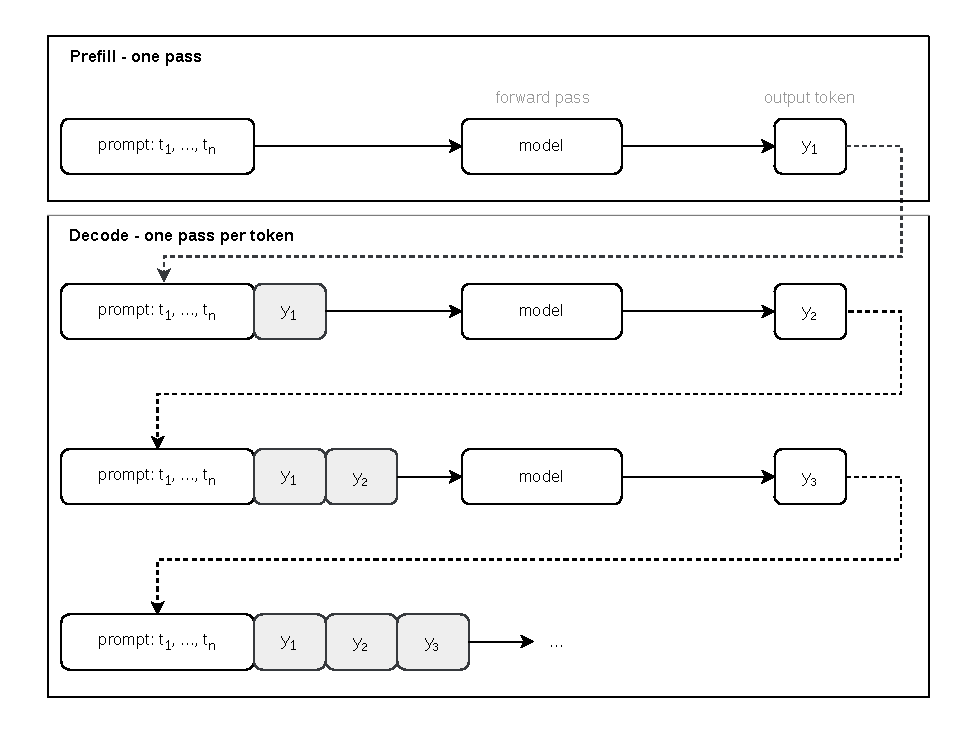
\includegraphics[width=0.9\textwidth]{images/prefill_decode.pdf}
	\caption[Prefill and decode]{Prefill and decode. Prefill processes the whole prompt in a single forward pass and emits the first token. Decode performs one forward pass per token, each time on the input extended by the token emitted at the previous step.}
	\label{fig:prefill-decode}
\end{figure}

The keys and values computed during prefill and at each decode step are stored in the key-value cache \cite{xuKVCacheOptimization2026}. Each decode step then computes attention only for the new token, using the cached keys and values, instead of recomputing attention for all previous tokens.

The distinction between prefill and decode matters for cost. The vectors produced at the last prompt token are produced by the prefill pass, which is executed in any case before the first output token can be emitted. Obtaining them therefore requires no additional forward pass, and no generated tokens. A method that reads the prefill representation and a method that reads the generated text differ in when they can act: the first can act before decoding begins, the second only after it has finished.
